% Slide 50: Density-based: LOF approach
\begin{frame}{ضریب ناهنجاری محلی (\lr{LOF}) مبتنی بر چگالی}{\lr{Density-based Outlier Detection: LOF}}
  \begin{itemize}
    \setlength{\itemsep}{5pt}
    \item برای هر نقطه، \textbf{چگالی همسایگی محلی} آن محاسبه می‌شود:
    \begin{itemize}
      \setlength{\itemsep}{3pt}
      \item اگر این چگالی بیشتر از میانگین چگالی همسایگان باشد، نقطه درون یک خوشه متراکم قرار دارد.
      \item اگر چگالی محلی به طور محسوسی کمتر از میانگین چگالی همسایگان باشد، نقطه یک \textbf{داده پرت} است.
    \end{itemize}
    \item \textbf{ضریب ناهنجاری محلی (\lr{Local Outlier Factor - LOF}):}
    \begin{itemize}
      \item نسبت میانگین چگالی همسایگان نقطه $A$ به چگالی خود نقطه $A$.
      \item نقاط نرمال و درون‌خوشه‌ای: $\text{LOF} \approx 1$
      \item نقاط پرت و ناهنجار: دارای $\text{LOF} > 1$ (به شکل معنادار بزرگ‌تر از ۱).
    \end{itemize}
  \end{itemize}
\end{frame}

% Slide 51: LOF Illustration
\begin{frame}{تصویرسازی مفهوم ضریب ناهنجاری محلی (\lr{LOF})}{\lr{LOF: Conceptual Illustration}}
  \begin{columns}[T]
    \begin{column}{0.54\textwidth}
      \begin{itemize}
        \setlength{\itemsep}{5pt}
        \item با در نظر گرفتن $k=3$ نزدیک‌ترین همسایه:
        \item مقادیر زیر محاسبه می‌شوند:
        \begin{itemize}
          \item چگالی محلی نقطه $A$.
          \item میانگین چگالی ۳ همسایه نزدیک به $A$.
        \end{itemize}
        \item نقطه $A$ نسبت به همسایگانش در فضایی بسیار خلوت‌تر قرار گرفته است:
        \begin{itemize}
          \item چگالی $A$ بسیار کمتر از چگالی همسایگان آن است.
          \item بنابراین نسبت $\text{LOF}(A) \gg 1$ شده و نقطه $A$ به عنوان داده پرت شناسایی می‌شود.
        \end{itemize}
      \end{itemize}
    \end{column}
    \begin{column}{0.44\textwidth}
      \begin{center}
        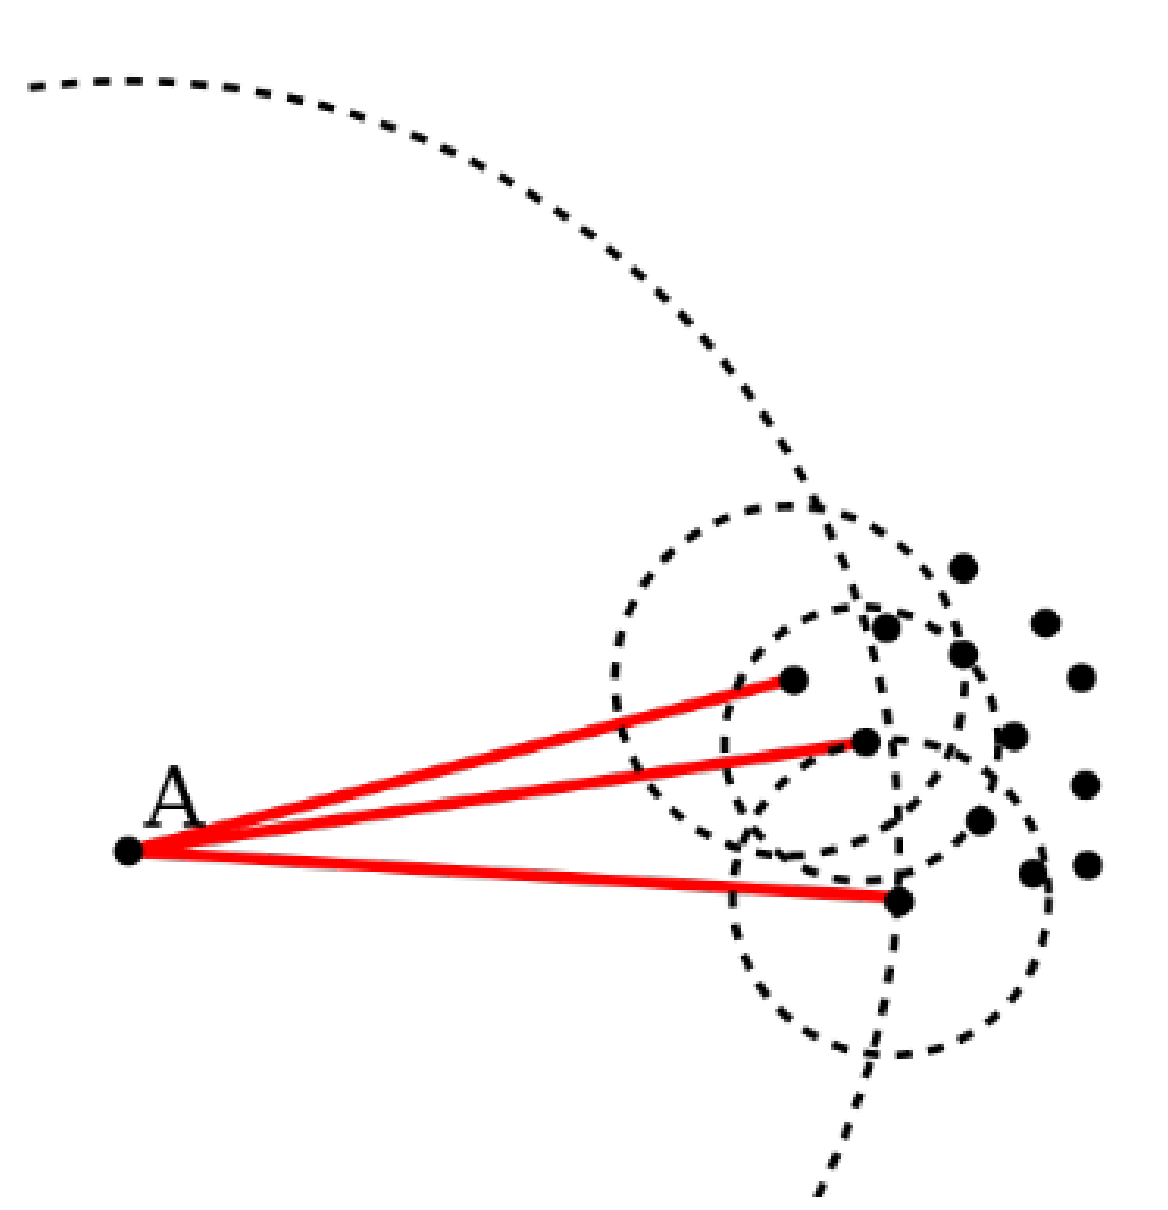
\includegraphics[width=\textwidth,height=4.8cm,keepaspectratio]{images/slide51_lof_illustration.png}
      \end{center}
    \end{column}
  \end{columns}
\end{frame}

% Slide 52: DBSCAN for Outlier Detection
\begin{frame}{کاربرد الگوریتم \lr{DBSCAN} در تشخیص داده‌های پرت}{\lr{DBSCAN for Outlier Detection}}
  \begin{columns}[c]
    \begin{column}{0.60\textwidth}
      \begin{itemize}
        \setlength{\itemsep}{4pt}
        \item الگوریتم \lr{DBSCAN} مستقیماً نقاط نویز را شناسایی می‌کند:
        \begin{itemize}
          \item این نقاط به هیچ خوشه‌ای تعلق ندارند (داده‌های پرت).
          \item در کتابخانه \lr{scikit-learn}: برچسب عددی $-1$ دریافت می‌کنند.
        \end{itemize}
        \item این قابلیت امکان تشخیص مستقیم داده‌های پرت را فراهم می‌سازد.
      \end{itemize}
    \end{column}
    \begin{column}{0.38\textwidth}
      \begin{center}
        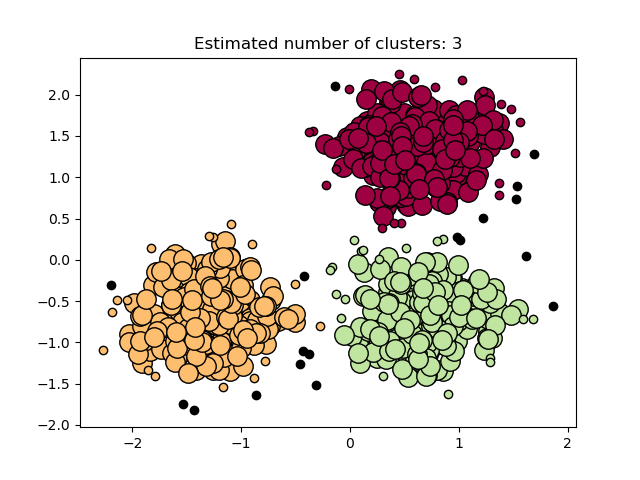
\includegraphics[width=\textwidth,height=2.7cm,keepaspectratio]{images/slide52_dbscan_clustering_plot.png}
      \end{center}
    \end{column}
  \end{columns}
  \vspace{0.15cm}
  \begin{center}
    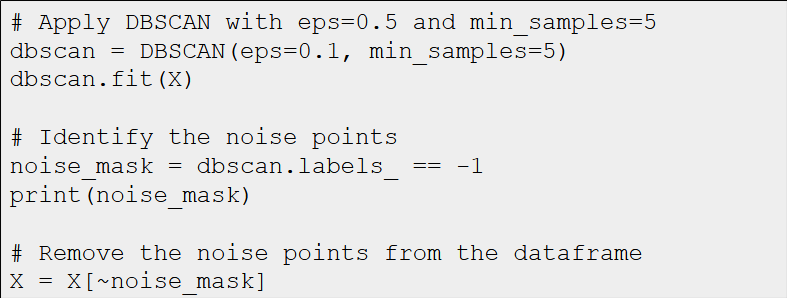
\includegraphics[width=0.96\textwidth,height=2.3cm,keepaspectratio]{images/slide52_dbscan_code.png}
  \end{center}
\end{frame}

% Slide 53: Clustering-based Outlier Detection
\begin{frame}{تشخیص داده‌های پرت مبتنی بر خوشه‌بندی}{\lr{Clustering-based Outlier Detection}}
  \begin{columns}[T]
    \begin{column}{0.54\textwidth}
      \textbf{ایده بنیادی:}
      \begin{itemize}
        \setlength{\itemsep}{4pt}
        \item ۱. خوشه‌بندی داده‌ها به گروه‌هایی با چگالی و اندازه متفاوت.
        \item ۲. انتخاب داده‌های متعلق به خوشه‌های بسیار کوچک به عنوان کاندیدای ناهنجاری.
        \item ۳. محاسبه فاصله میان نقاط کاندیدا و خوشه‌های اصلی بزرگ.
        \item ۴. اگر نقاط کاندیدا فاصله زیادی از سایر خوشه‌ها داشته باشند، رسماً به عنوان دادۀ پرت برچسب می‌خورند.
      \end{itemize}
    \end{column}
    \begin{column}{0.44\textwidth}
      \begin{center}
        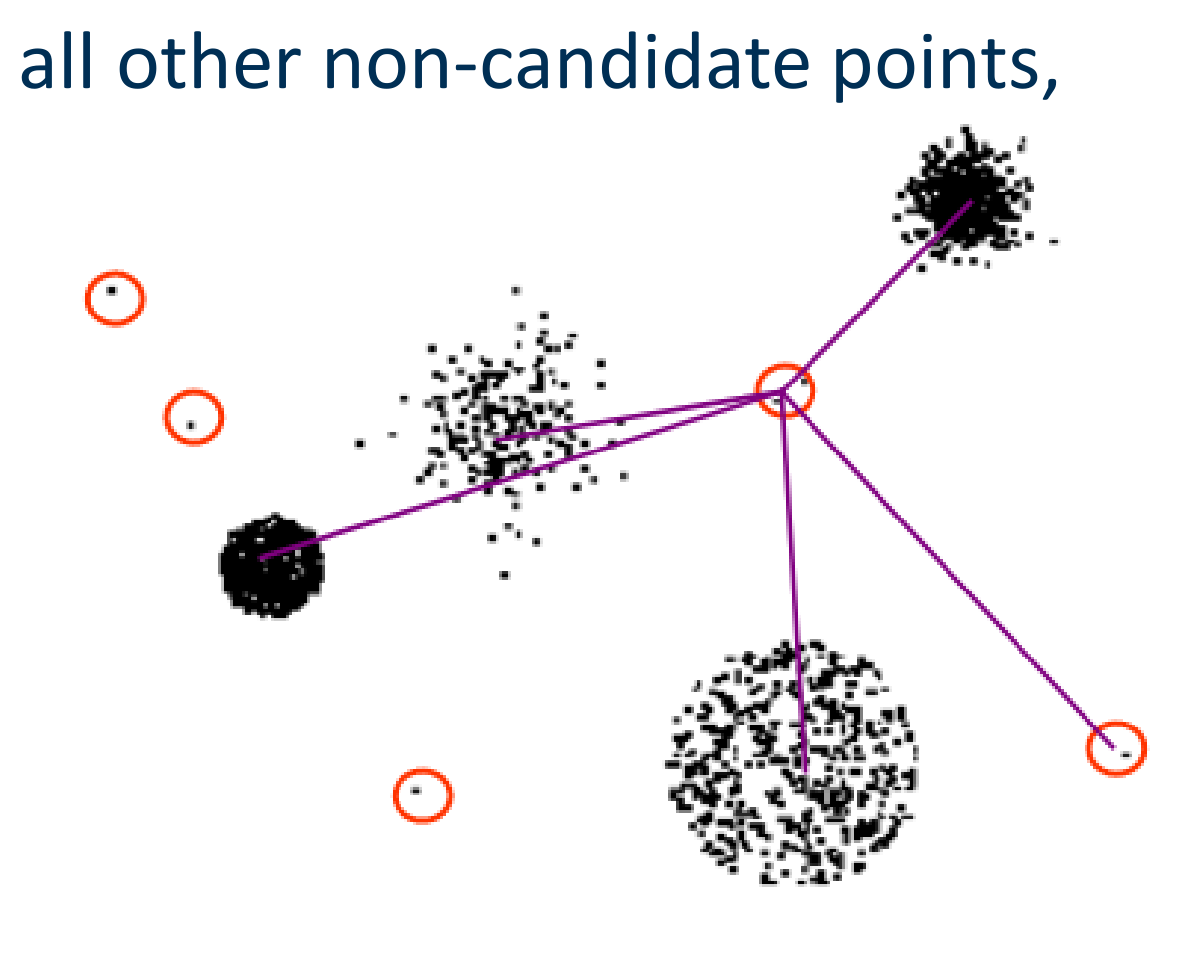
\includegraphics[width=\textwidth,height=4.6cm,keepaspectratio]{images/slide53_clustering_outliers.png}
      \end{center}
    \end{column}
  \end{columns}
\end{frame}

% Slide 54: CBLOF
\begin{frame}{ضریب ناهنجاری محلی مبتنی بر خوشه (\lr{CBLOF})}{\lr{Clustering-based Local Outlier Factor (CBLOF)}}
  \begin{columns}[T]
    \begin{column}{0.54\textwidth}
      \begin{itemize}
        \setlength{\itemsep}{5pt}
        \item \textbf{تعریف ناهنجاری در الگوریتم \lr{CBLOF}:}
        \begin{itemize}
          \item قرارگیری در یک خوشه بسیار کوچک.
          \item یا داشتن فاصله زیاد تا سایر خوشه‌های اصلی داده‌ها.
        \end{itemize}
        \item این معیار پس از اجرای یک الگوریتم خوشه‌بندی اولیه روی داده‌ها اعمال می‌شود.
        \item \textbf{امتیازدهی نهایی بر اساس دو عامل:}
        \begin{enumerate}
          \item اندازه خوشه‌ای که نقطه داده در آن قرار دارد.
          \item فاصله نقطه داده تا نزدیک‌ترین خوشه بزرگ.
        \end{enumerate}
      \end{itemize}
    \end{column}
    \begin{column}{0.44\textwidth}
      \begin{center}
        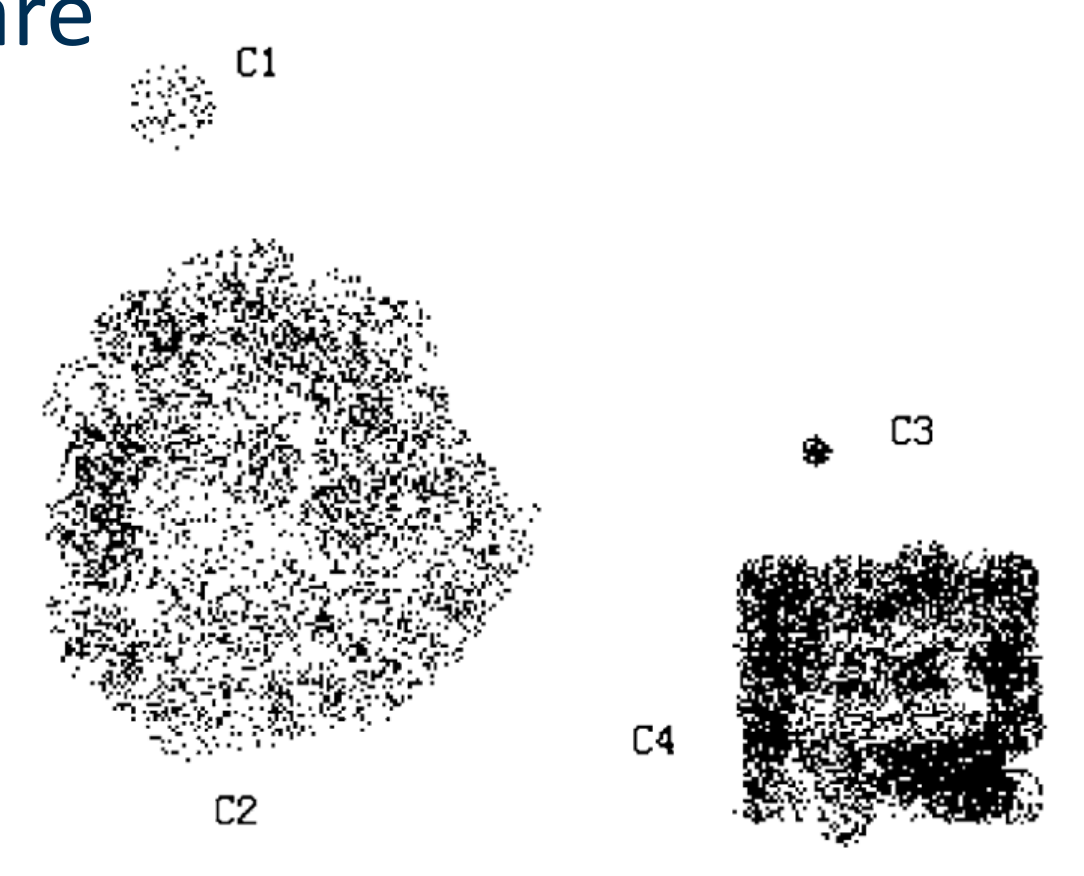
\includegraphics[width=\textwidth,height=4.6cm,keepaspectratio]{images/slide54_cblof_diagram.png}
      \end{center}
    \end{column}
  \end{columns}
\end{frame}

% Slide 55: CBLOF Workflow
\begin{frame}{فرایند اجرایی الگوریتم \lr{CBLOF} و بسته \lr{PyOD}}{\lr{CBLOF Workflow \& PyOD}}
  \begin{columns}[T]
    \begin{column}{0.55\textwidth}
      \begin{itemize}
        \setlength{\itemsep}{6pt}
        \item \textbf{مراحل گام‌به‌گام فرایند:}
        \begin{enumerate}
          \setlength{\itemsep}{3pt}
          \item اجرای یک الگوریتم خوشه‌بندی دلخواه (مانند \lr{K-Means} یا \lr{DBSCAN}).
          \item تفکیک خوشه‌ها به خوشه‌های بزرگ \lr{(Large)} و کوچک \lr{(Small)}.
          \item اعمال الگوریتم \lr{CBLOF} بر روی نتایج حاصل.
        \end{enumerate}
        \item \textbf{خروجی:} انتساب یک امتیاز پیوسته ناهنجاری \lr{(Outlier Score)} به تک‌تک نمونه‌های داده.
        \item پیاده‌سازی رسمی و بهینه‌سازی‌شده این روش در کتابخانه \lr{PyOD} در دسترس است.
      \end{itemize}
    \end{column}
    \begin{column}{0.42\textwidth}
      \begin{center}
        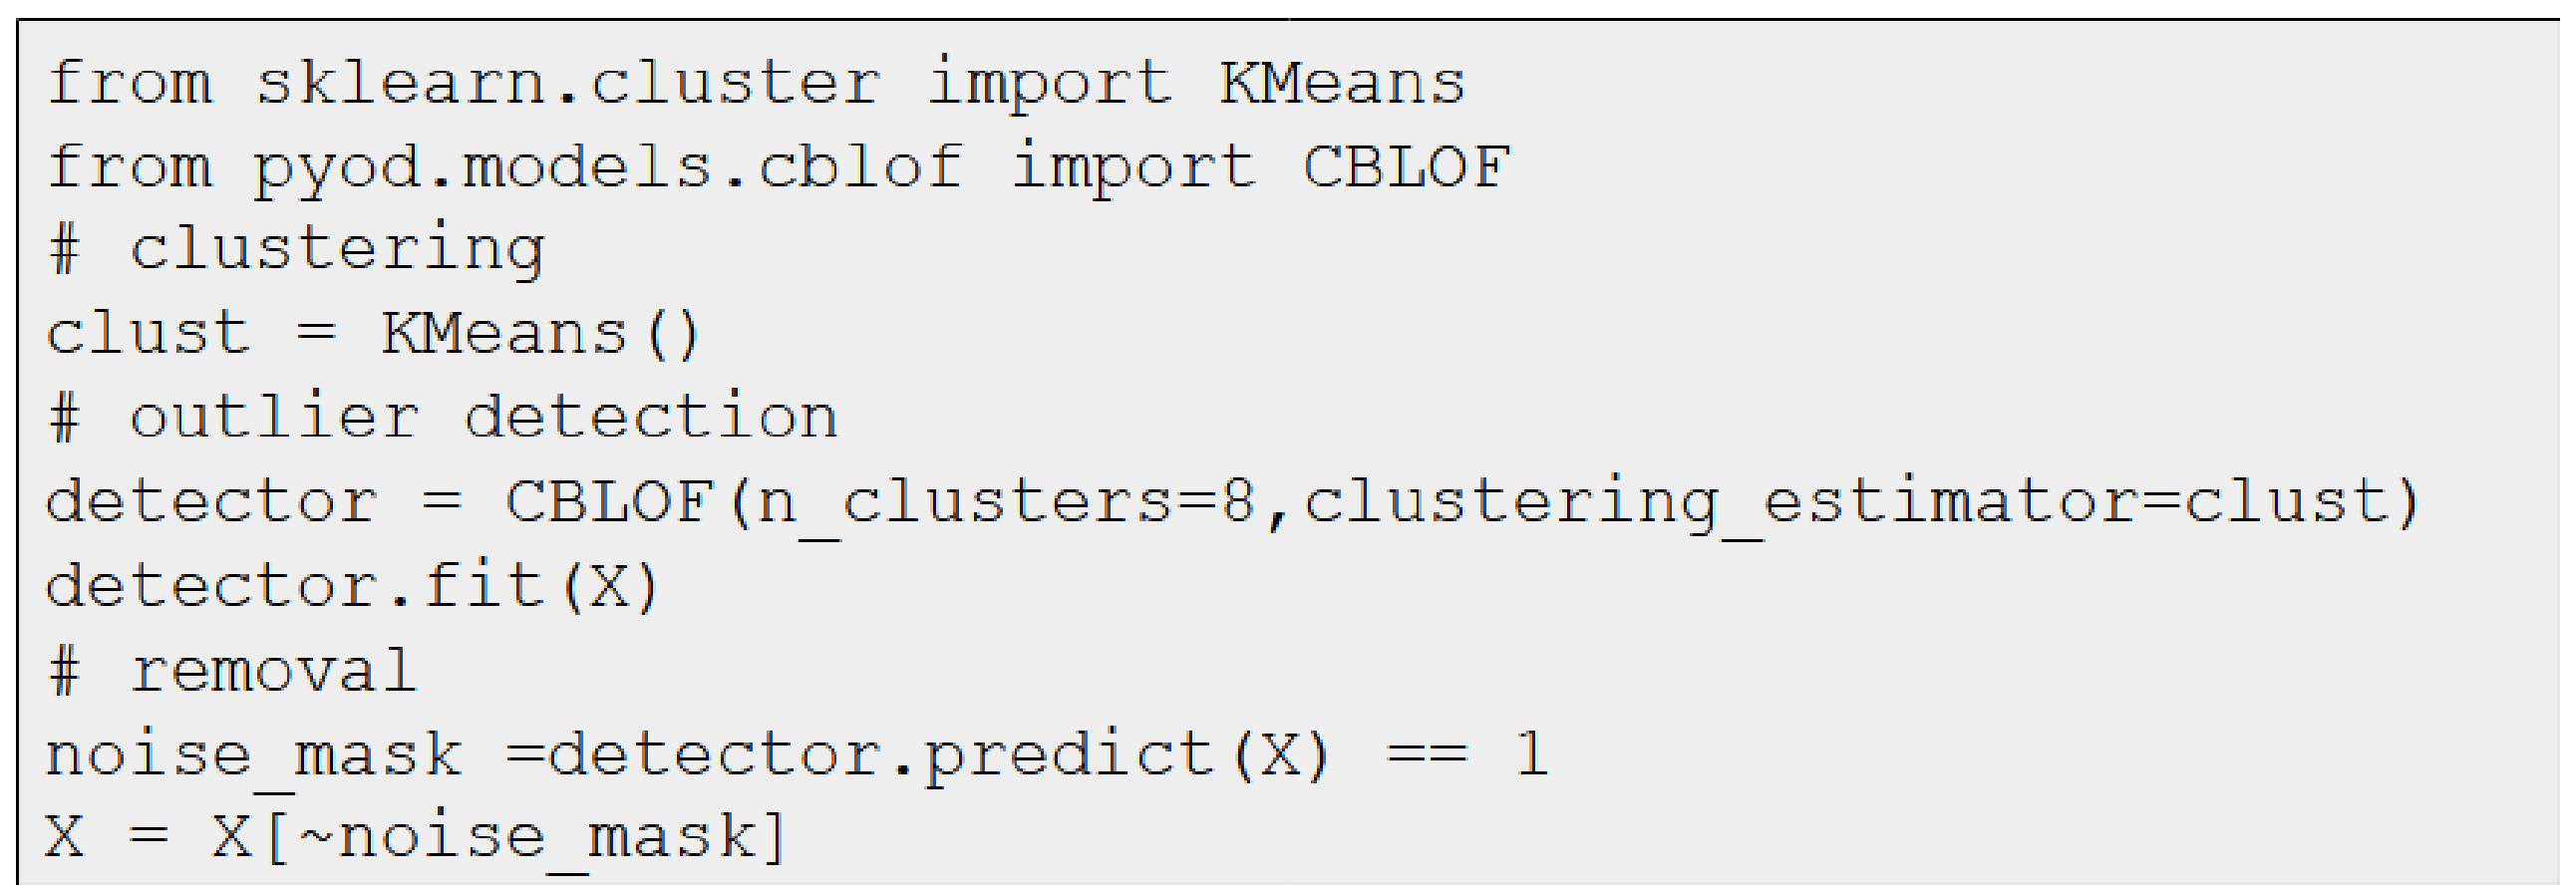
\includegraphics[width=\textwidth,height=4.4cm,keepaspectratio]{images/slide55_cblof_evaluation.png}
      \end{center}
    \end{column}
  \end{columns}
\end{frame}

% Slide 56: Isolation Forest Concepts
\begin{frame}{مفاهیم پایه در الگوریتم جنگل انزوا (\lr{Isolation Forest})}{\lr{Isolation Forest: Basic Concepts}}
  \begin{columns}[T]
    \begin{column}{0.52\textwidth}
      \begin{itemize}
        \setlength{\itemsep}{4pt}
        \item \textbf{درخت انزوا:} \lr{(Isolation Tree - iTree)}
        \begin{itemize}
          \item یک درخت تصمیم که هر برگ آن در نهایت شامل تنها \textbf{یک نمونه داده} است.
        \end{itemize}
        \item \textbf{جنگل انزوا:} \lr{(Isolation Forest - iForest)}
        \begin{itemize}
          \item آموزش مجموعه‌ای (گروهی) از درخت‌های انزوای تصادفی.
        \end{itemize}
        \item \textbf{شهود کلیدی:}
        \begin{itemize}
          \item مسیر رسیدن به نقاط پرت در درخت \textbf{بسیار کوتاه‌تر} از نقاط عادی است (سریع‌تر منزوی می‌شوند).
          \item میانگین طول مسیر در میان درختان، معیار امتیاز ناهنجاری است.
        \end{itemize}
      \end{itemize}
    \end{column}
    \begin{column}{0.46\textwidth}
      \begin{center}
        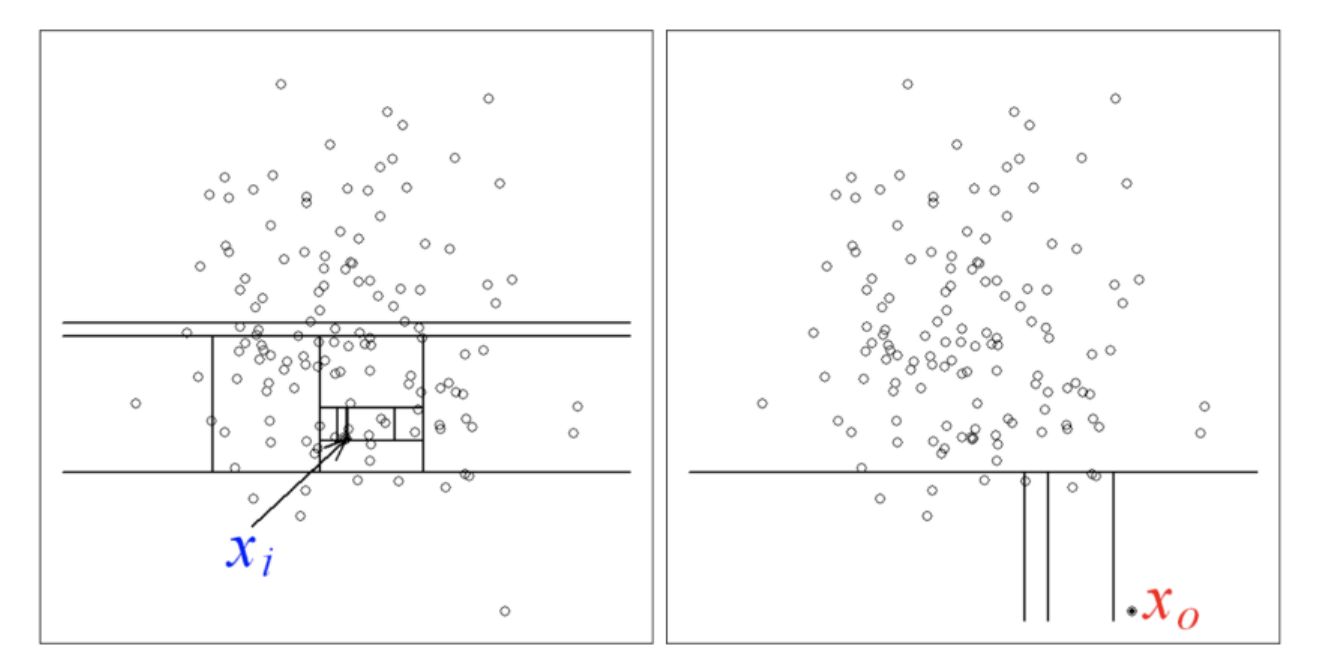
\includegraphics[width=\textwidth,height=2.3cm,keepaspectratio]{images/slide56_isolation_forest_concept1.png}\\[0.15cm]
        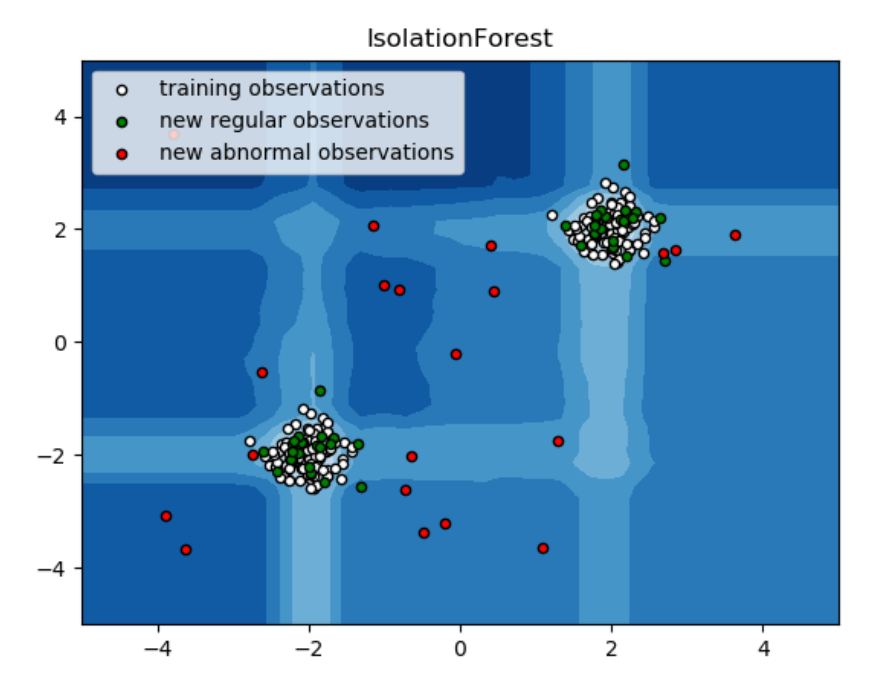
\includegraphics[width=\textwidth,height=2.3cm,keepaspectratio]{images/slide56_isolation_forest_concept2.png}
      \end{center}
    \end{column}
  \end{columns}
\end{frame}

% Slide 57: Isolation Forest Training
\begin{frame}{آموزش یک درخت انزوا}{\lr{Training a Single Isolation Tree}}
  \begin{columns}[T]
    \begin{column}{0.54\textwidth}
      \begin{itemize}
        \setlength{\itemsep}{4pt}
        \item \textbf{فرایند تقسیم در هر گره برگ (با بیش از ۱ داده):}
        \begin{itemize}
          \setlength{\itemsep}{2pt}
          \item انتخاب تصادفی یکی از ویژگی‌ها \lr{(Att)}.
          \item انتخاب تصادفی یک مقدار برش \lr{(V)} در بازه تغییرات آن ویژگی.
          \item ایجاد گره درونی با شرط آزمون $\text{Att} < V$.
        \end{itemize}
        \item تکرار بازگشتی فرایند ساخت برای هر زیردرخت.
        \item \textbf{خروجی:} درختی که در هر گره برگ نهایی آن فقط ۱ نمونه وجود دارد (معمولاً سقف ارتفاعی برای کارایی تعیین می‌شود).
      \end{itemize}
    \end{column}
    \begin{column}{0.44\textwidth}
      \begin{center}
        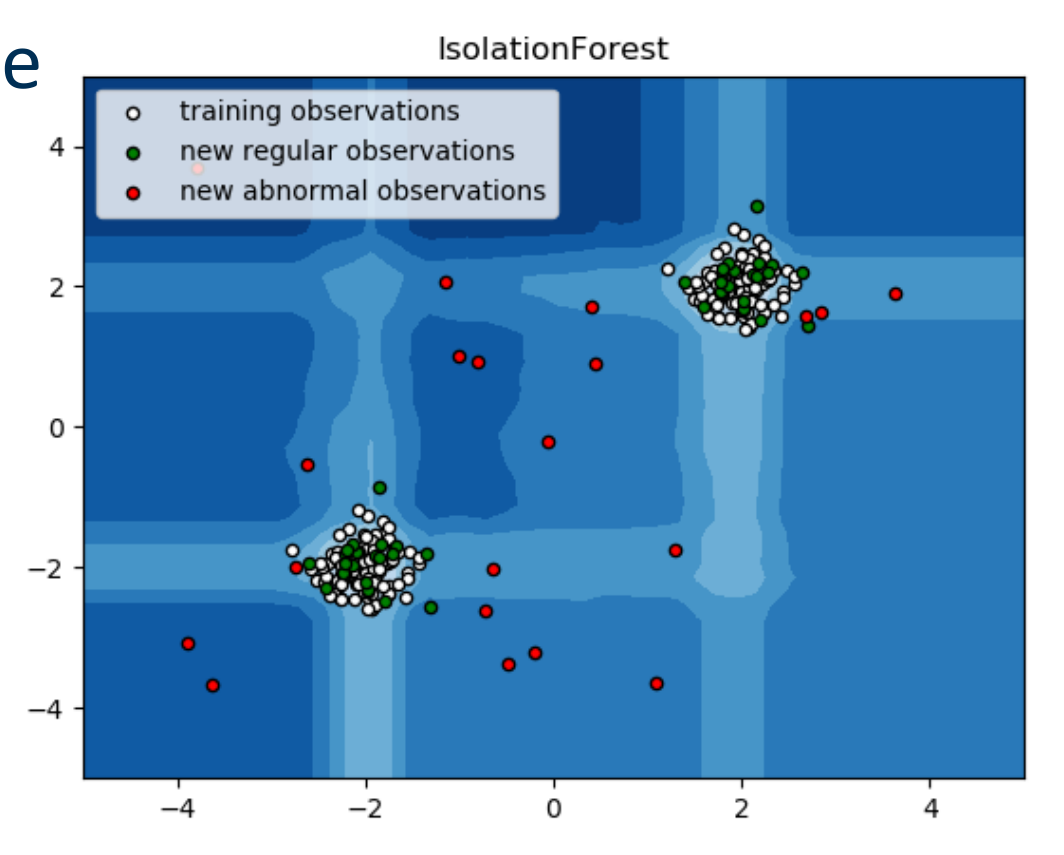
\includegraphics[width=\textwidth,height=4.6cm,keepaspectratio]{images/slide57_iforest_partitioning.png}
      \end{center}
    \end{column}
  \end{columns}
\end{frame}

% Slide 58: Step 1
\begin{frame}{محاسبه احتمال انزوای نقطه دورافتاده در ارتفاع اول}{\lr{Isolation Forest: Probability of (0,0) at Height 1}}
  \begin{columns}[T]
    \begin{column}{0.60\textwidth}
      {\fontsize{8.5}{11.5}\selectfont
      \begin{itemize}
        \setlength{\itemsep}{4pt}
        \item نقطه دورافتاده با مختصات $(0,0)$ در گوشه پایین سمت چپ را در نظر بگیرید.
        \item احتمال انزوای این نقطه با \textbf{تنها یک برش} در ارتفاع ۱:
        \item \textbf{حالت اول:}
        \begin{itemize}
          \setlength{\itemsep}{2pt}
          \item انتخاب ویژگی $X$ (احتمال $0.5$).
          \item انتخاب مقدار برش در بازه $X < 0.52$ (احتمال $0.52$).
        \end{itemize}
        \item این برش نقطه $(0,0)$ را فوراً از تمامی داده‌های دیگر جدا می‌کند.
      \end{itemize}
      }
    \end{column}
    \begin{column}{0.38\textwidth}
      \begin{center}
        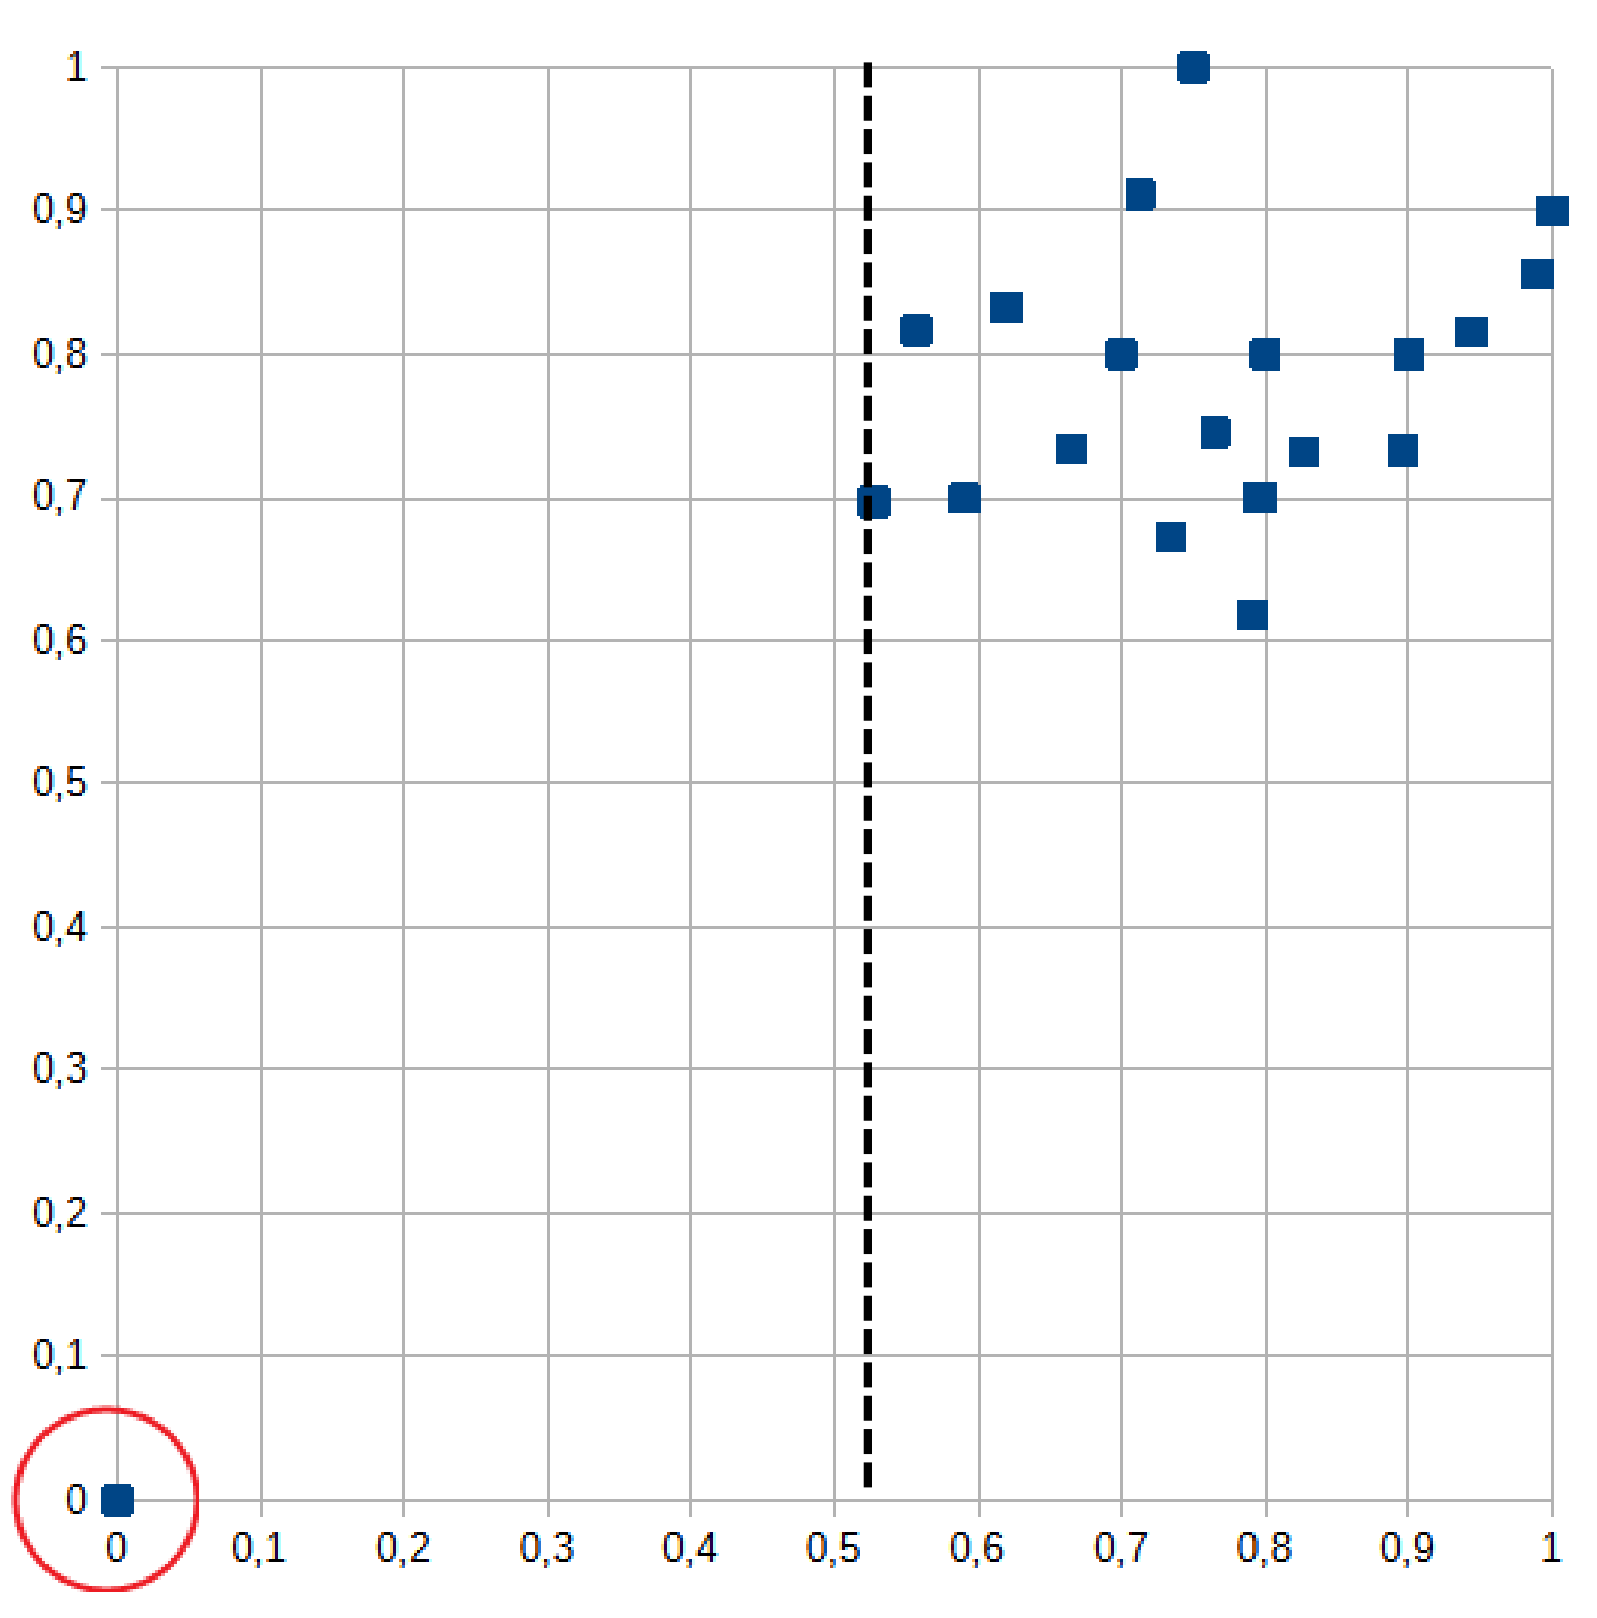
\includegraphics[width=\textwidth,height=4.6cm,keepaspectratio]{images/slide58_iforest_tree.png}
      \end{center}
    \end{column}
  \end{columns}
\end{frame}

% Slide 59: Step 2
\begin{frame}{احتمال کل انزوای نقطه دورافتاده در ارتفاع اول}{\lr{Isolation Forest: Total Probability for (0,0)}}
  \begin{columns}[T]
    \begin{column}{0.60\textwidth}
      {\fontsize{8.5}{11.5}\selectfont
      \begin{itemize}
        \setlength{\itemsep}{3pt}
        \item نقطه $(0,0)$ هم با برش روی محور $X$ و هم با برش روی محور $Y$ منزوی می‌شود:
        \begin{itemize}
          \setlength{\itemsep}{2pt}
          \item انتخاب محور $X$ و برش $X < 0.52$
          \item یا انتخاب محور $Y$ و برش $Y < 0.62$
        \end{itemize}
        \item \textbf{محاسبه احتمال کل:}
        \begin{center}
          \lr{\small $P = 0.5 \times 0.52 + 0.5 \times 0.62 = \mathbf{0.57}$}
        \end{center}
        \item بیش از $\%57$ احتمال دارد که این نقطه در \textbf{همان اولین برش} کاملاً جدا شود!
      \end{itemize}
      }
    \end{column}
    \begin{column}{0.38\textwidth}
      \begin{center}
        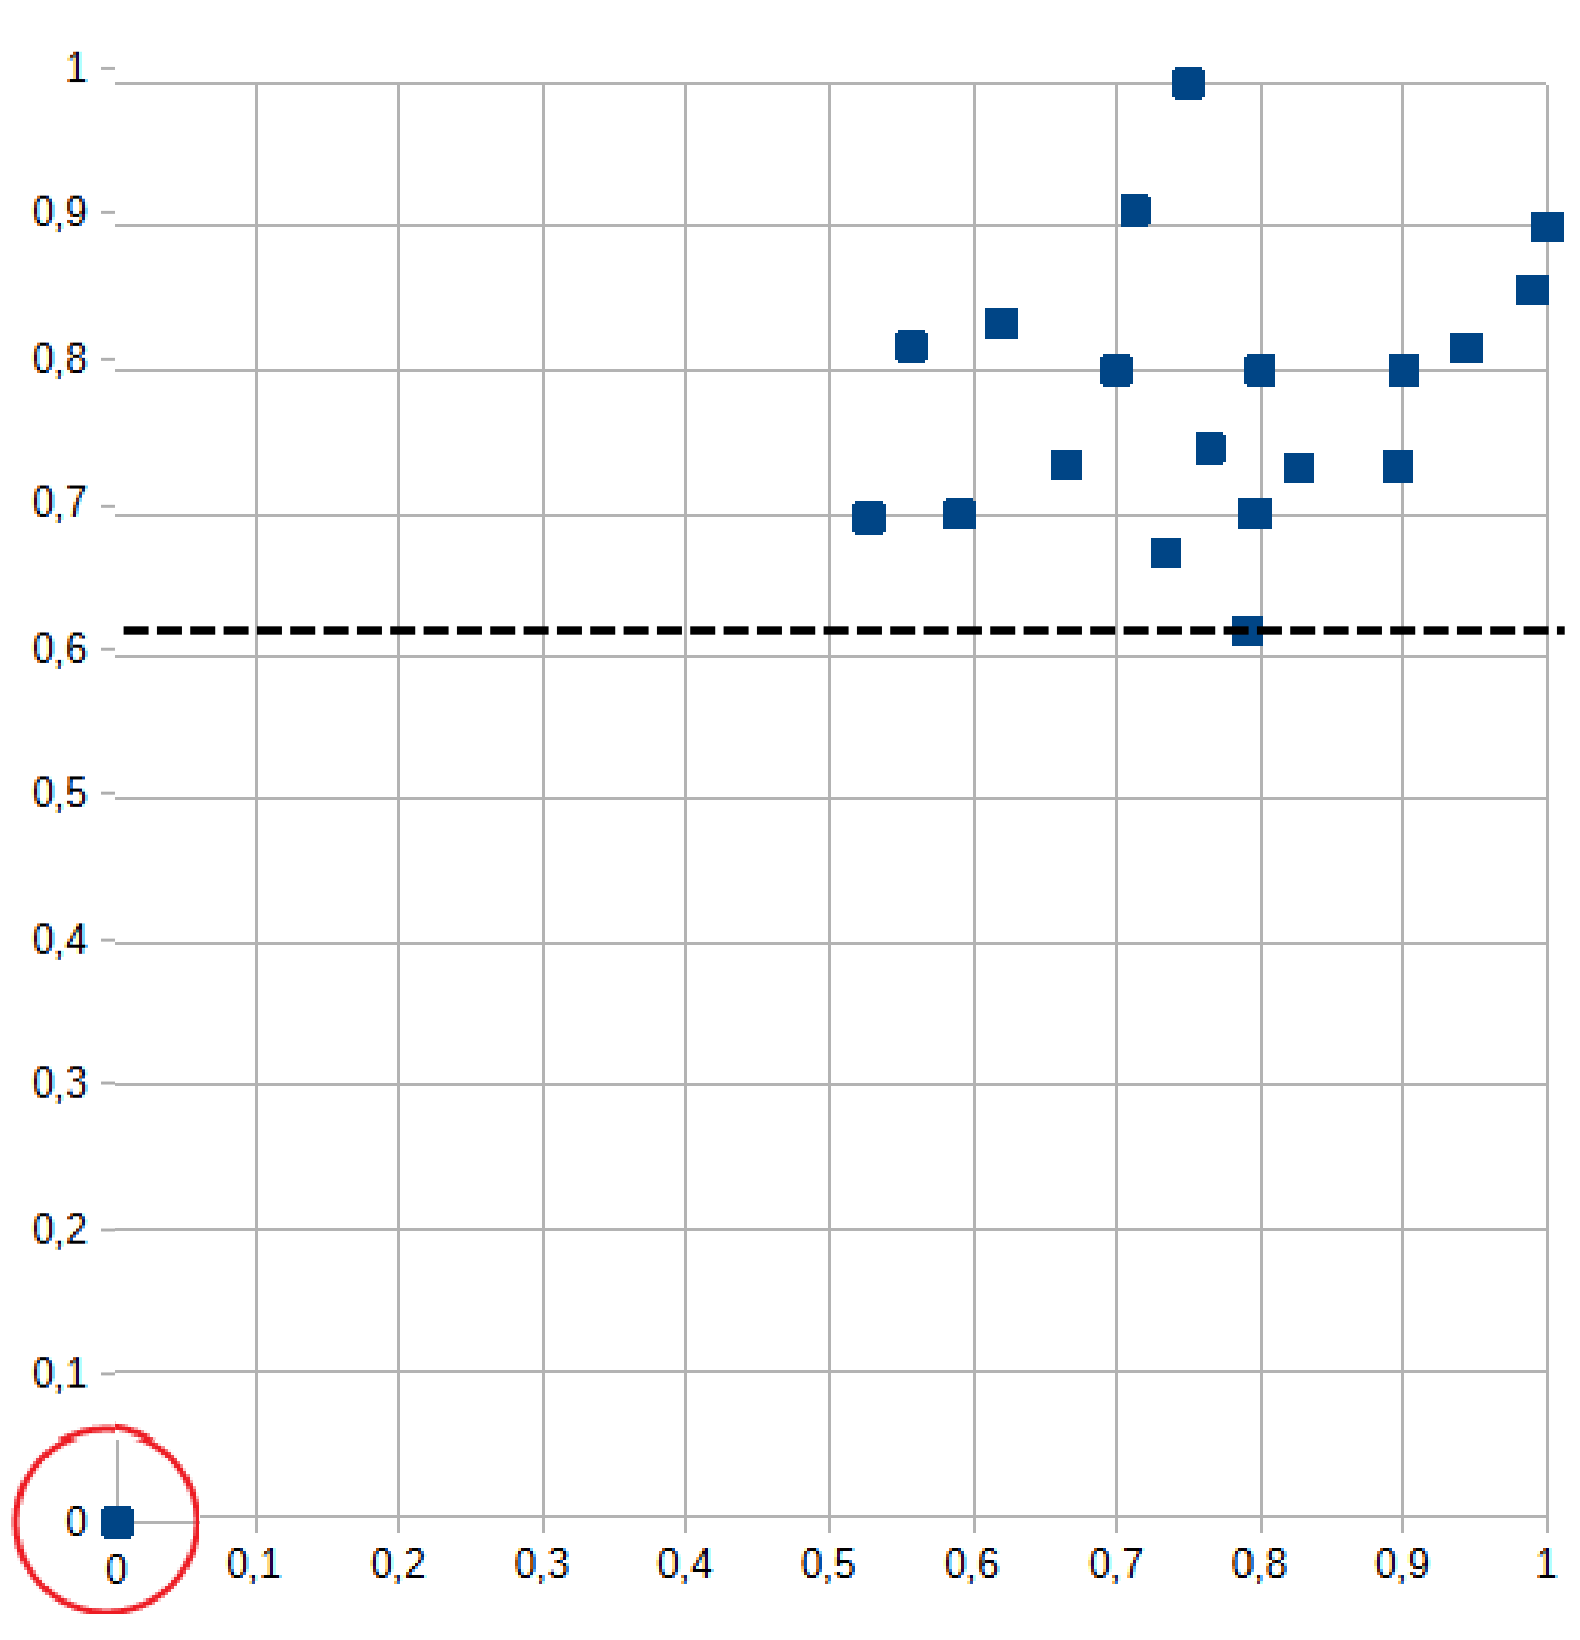
\includegraphics[width=\textwidth,height=4.6cm,keepaspectratio]{images/slide59_iforest_tree.png}
      \end{center}
    \end{column}
  \end{columns}
\end{frame}

% Slide 60: Step 3
\begin{frame}{احتمال انزوای نقطه شبه‌مرزی}{\lr{Isolation Forest: Probability of (0.74, 1)}}
  \begin{columns}[T]
    \begin{column}{0.60\textwidth}
      {\fontsize{8.5}{11.5}\selectfont
      \begin{itemize}
        \setlength{\itemsep}{4pt}
        \item بررسی احتمال انزوای نقطه شبه‌مرزی با مختصات $(0.74, 1)$ در ارتفاع ۱:
        \item تنها با برش روی ویژگی $Y$ و شرط $Y > 0.91$ منزوی می‌شود.
        \item \textbf{محاسبه احتمال:}
        \begin{center}
          \lr{\small $P = 0.5 \times (1 - 0.91) = 0.5 \times 0.09 = \mathbf{0.045}$}
        \end{center}
        \item این احتمال ($\%4.5$) بسیار کمتر از احتمال نقطه دورافتاده $(0,0)$ با $\%57$ است.
      \end{itemize}
      }
    \end{column}
    \begin{column}{0.38\textwidth}
      \begin{center}
        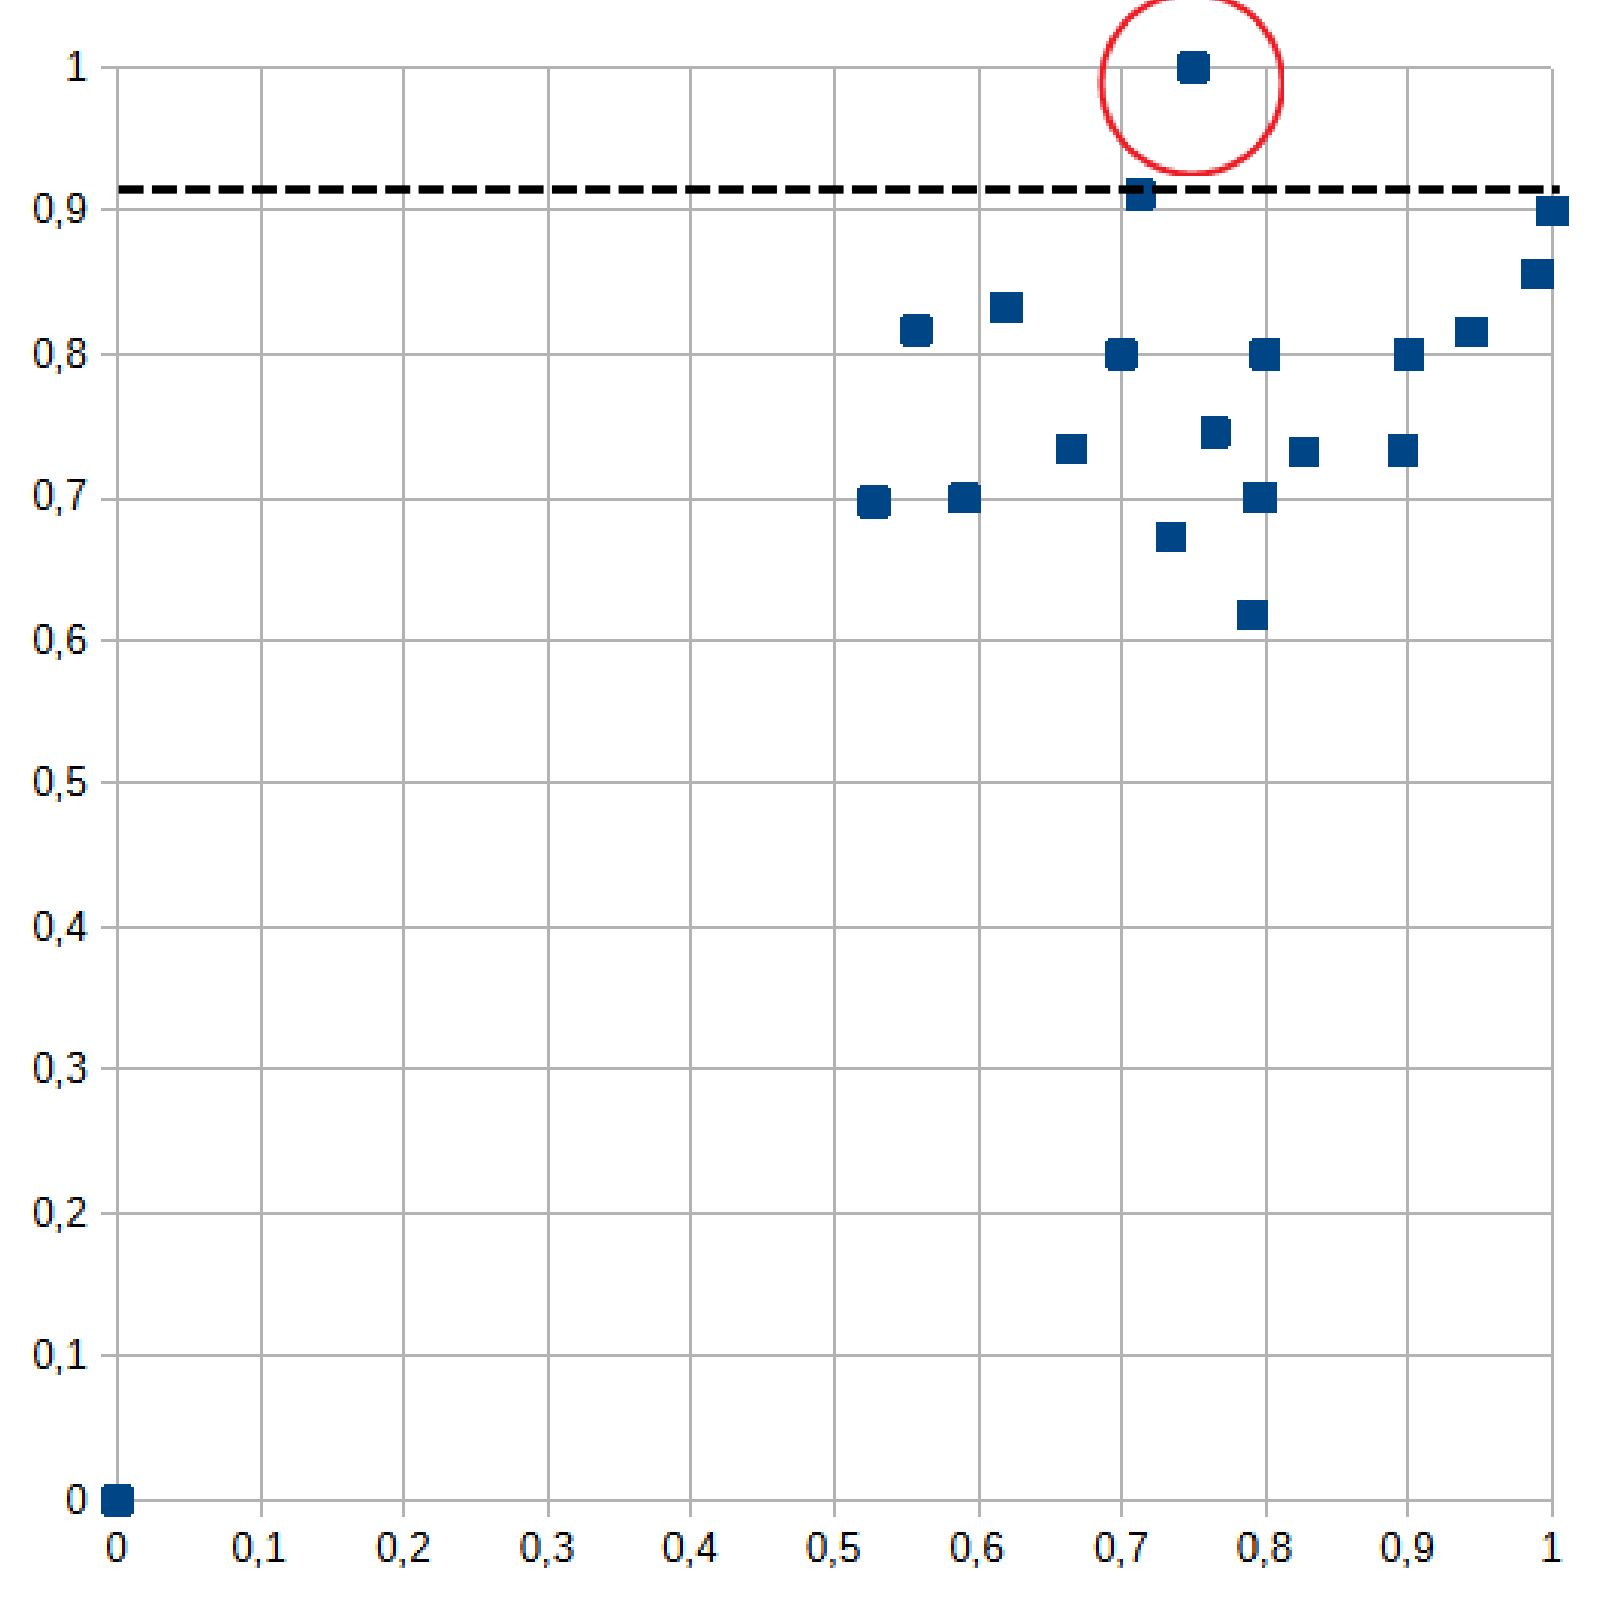
\includegraphics[width=\textwidth,height=4.6cm,keepaspectratio]{images/slide60_iforest_tree.png}
      \end{center}
    \end{column}
  \end{columns}
\end{frame}

% Slide 61: Step 4
\begin{frame}{احتمال انزوای نقطه مرزی}{\lr{Isolation Forest: Probability of (1, 0.9)}}
  \begin{columns}[T]
    \begin{column}{0.60\textwidth}
      {\fontsize{8.5}{11.5}\selectfont
      \begin{itemize}
        \setlength{\itemsep}{4pt}
        \item بررسی احتمال انزوای نقطه مرزی دیگر با مختصات $(1, 0.9)$ در ارتفاع ۱:
        \item تنها با انتخاب ویژگی $X$ و مقدار برش $X > 0.98$ منزوی می‌شود.
        \item \textbf{محاسبه احتمال:}
        \begin{center}
          \lr{\small $P = 0.5 \times (1 - 0.98) = 0.5 \times 0.02 = \mathbf{0.01}$}
        \end{center}
        \item احتمال انزوا در گام اول تنها $\%1$ است.
      \end{itemize}
      }
    \end{column}
    \begin{column}{0.38\textwidth}
      \begin{center}
        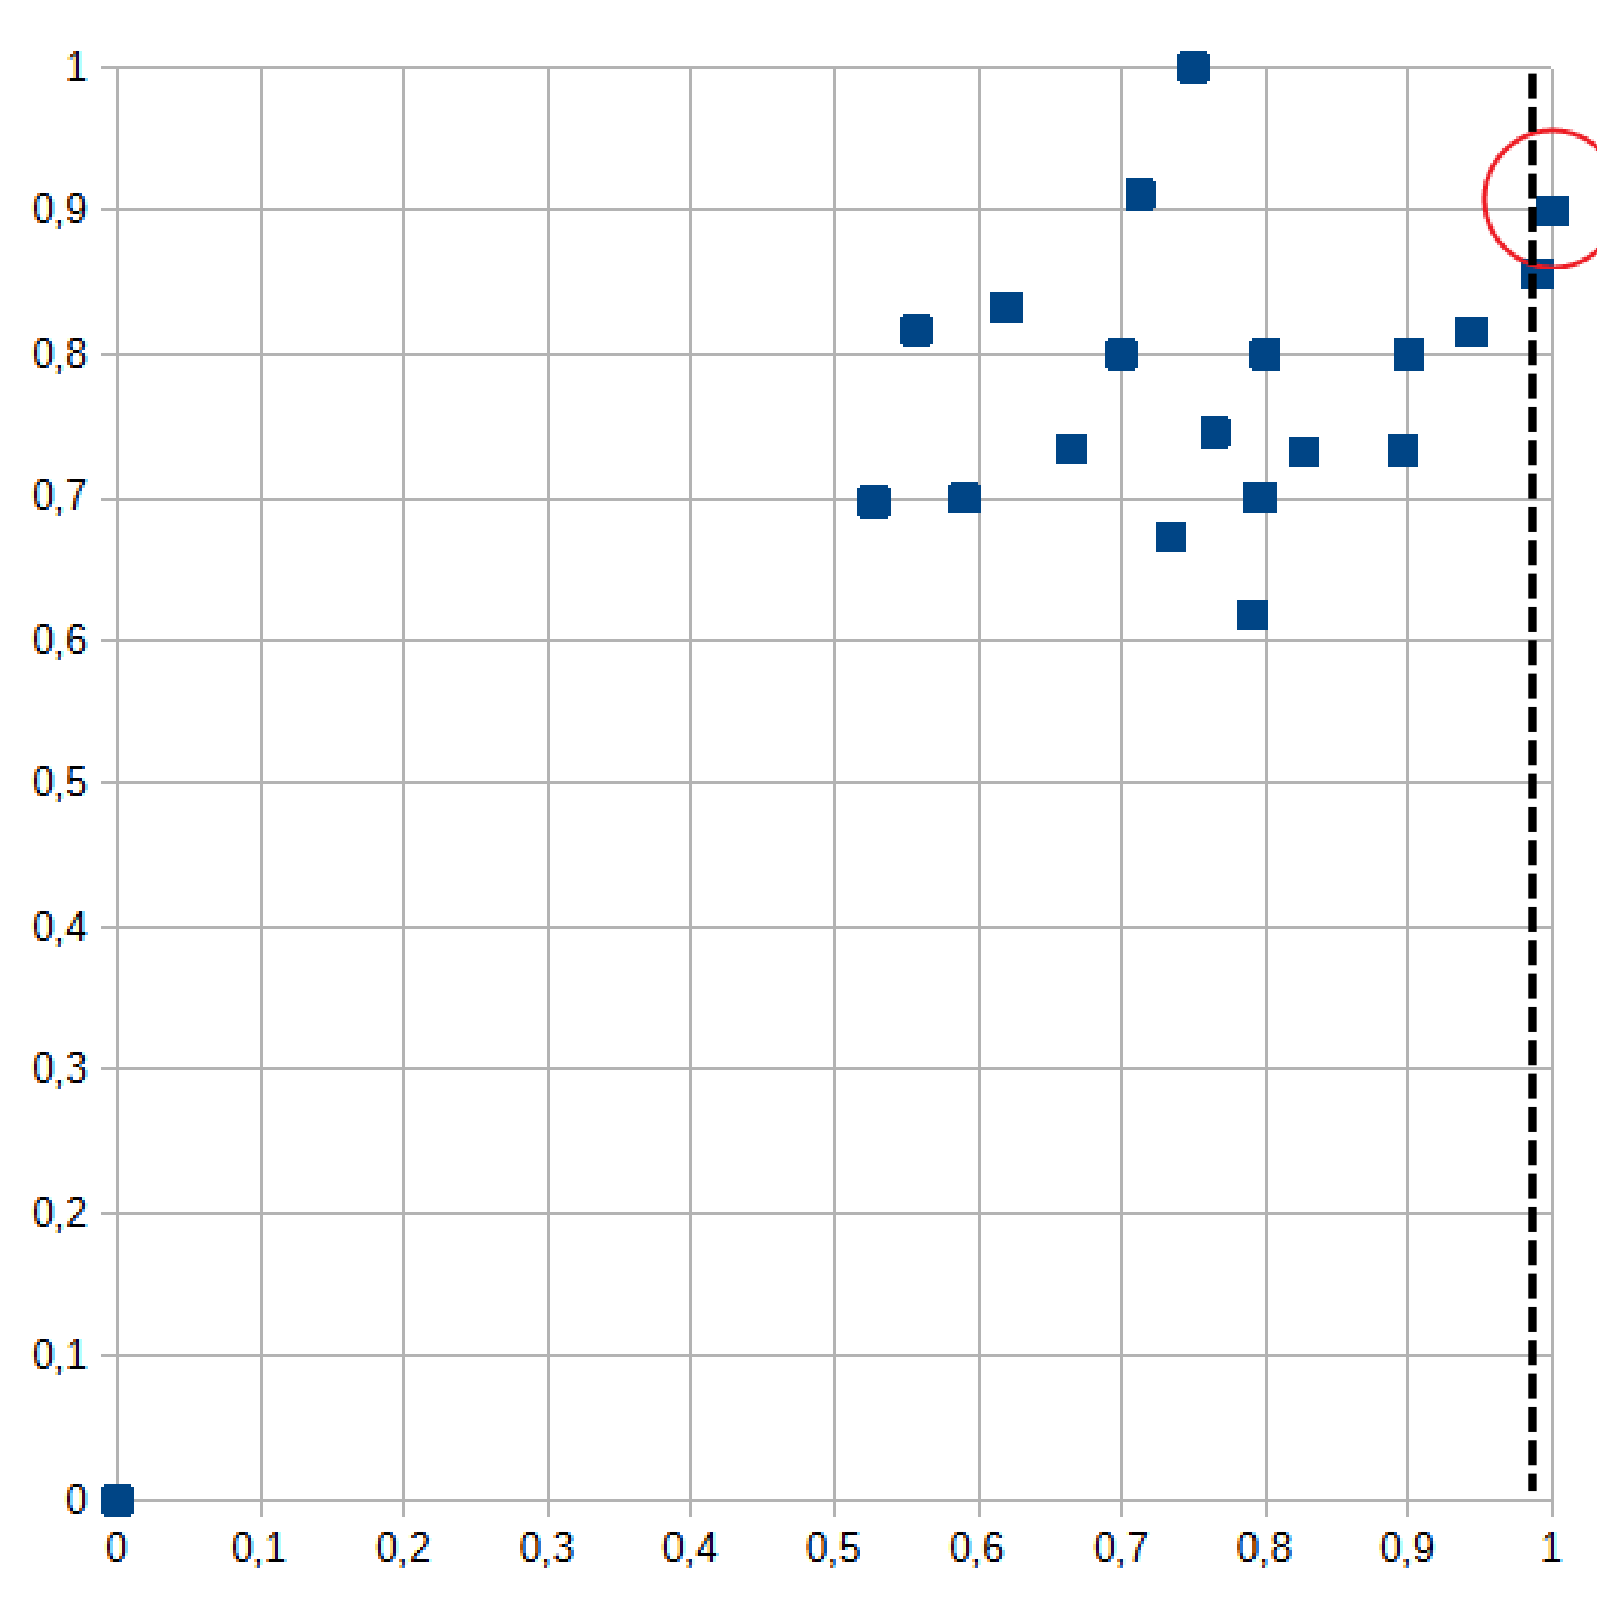
\includegraphics[width=\textwidth,height=4.6cm,keepaspectratio]{images/slide61_iforest_tree.png}
      \end{center}
    \end{column}
  \end{columns}
\end{frame}

% Slide 62: Step 5
\begin{frame}{احتمال انزوای سایر نقاط داده در ارتفاع اول}{\lr{Isolation Forest: Other Data Points}}
  \begin{columns}[T]
    \begin{column}{0.60\textwidth}
      {\fontsize{8.5}{11.5}\selectfont
      \begin{itemize}
        \setlength{\itemsep}{4pt}
        \item \textbf{احتمال انزوای سایر نقاط داده در ارتفاع ۱:}
        \begin{itemize}
          \setlength{\itemsep}{2pt}
          \item برای تمام نقاط دیگر داده که در ناحیه متراکم قرار دارند، انزوا در ارتفاع ۱ \textbf{غیرممکن است} ($P = 0$).
          \item برای جداسازی این نقاط حداقل به دو یا چند تقسیم متوالی نیاز است.
        \end{itemize}
        \item این امر نشان می‌دهد نقاط درونی هرگز در سطوح بالای درخت منزوی نمی‌شوند.
      \end{itemize}
      }
    \end{column}
    \begin{column}{0.38\textwidth}
      \begin{center}
        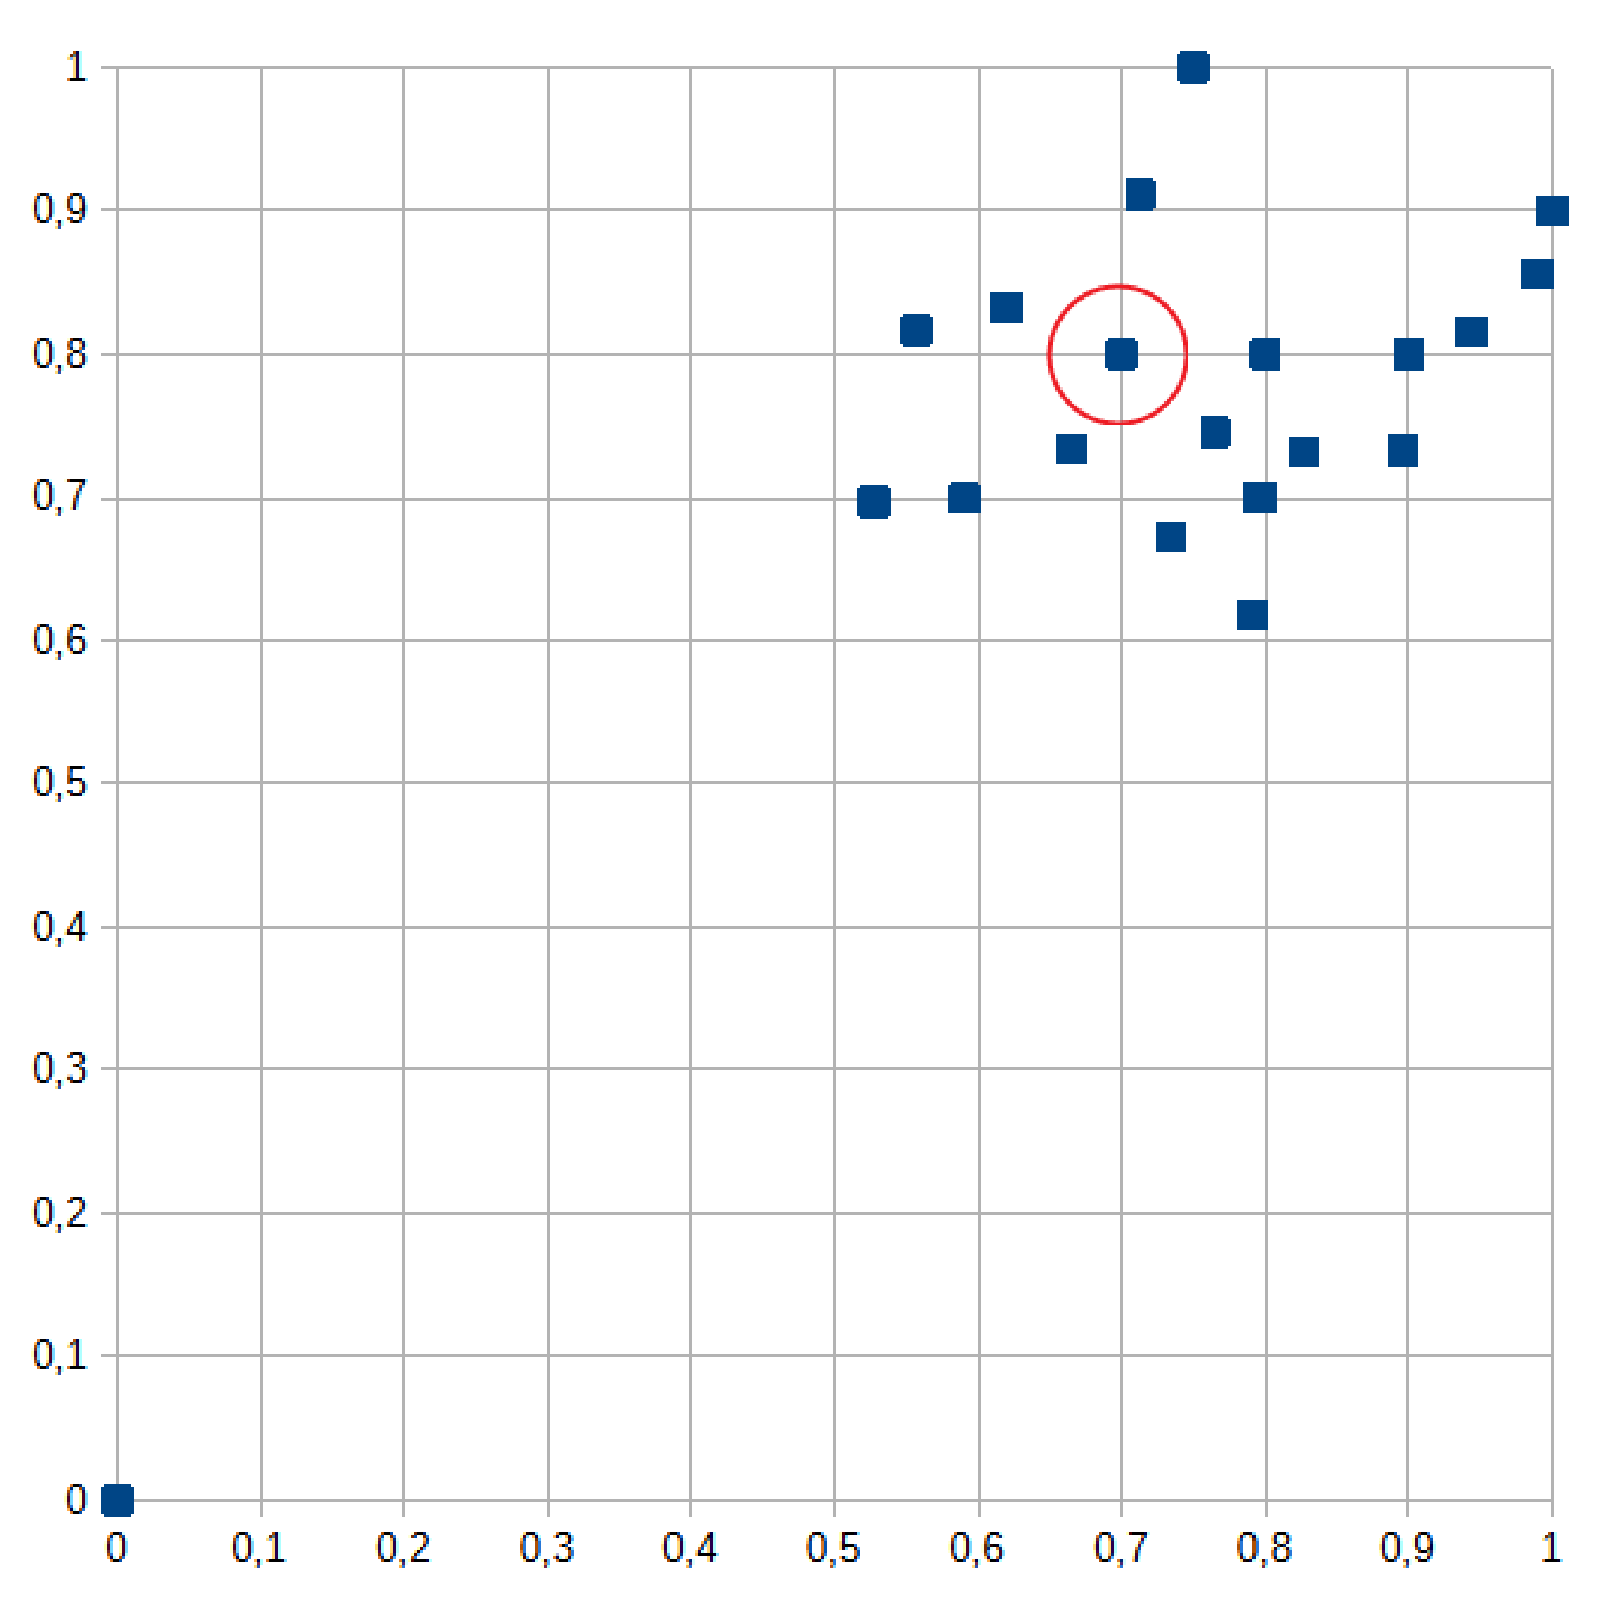
\includegraphics[width=\textwidth,height=4.6cm,keepaspectratio]{images/slide62_iforest_tree.png}
      \end{center}
    \end{column}
  \end{columns}
\end{frame}

% Slide 63: Isolation Forest Observations
\begin{frame}{مشاهدات و نتیجه‌گیری جنگل انزوا}{\lr{Isolation Forest: Key Observations}}
  \begin{columns}[T]
    \begin{column}{0.60\textwidth}
      {\fontsize{8.5}{11.5}\selectfont
      \begin{itemize}
        \setlength{\itemsep}{4pt}
        \item \textbf{نقاط در نواحی متراکم:} \lr{(Dense Areas)}
        \begin{itemize}
          \setlength{\itemsep}{2pt}
          \item نیازمند برش‌ها و آزمون‌های بسیار بیشتری هستند.
          \item در \textbf{عمق زیاد درخت} منزوی می‌شوند (طول مسیر بلند).
        \end{itemize}
        \item \textbf{نقاط پرت و دورافتاده:} \lr{(Outliers)}
        \begin{itemize}
          \setlength{\itemsep}{2pt}
          \item احتمال بسیار بالایی برای انزوای زودهنگام دارند.
          \item در \textbf{سطوح بالایی درخت} قرار می‌گیرند (طول مسیر کوتاه).
        \end{itemize}
        \item مرتبه خطی و کارایی بسیار بالا در داده‌های عظیم.
      \end{itemize}
      }
    \end{column}
    \begin{column}{0.38\textwidth}
      \begin{center}
        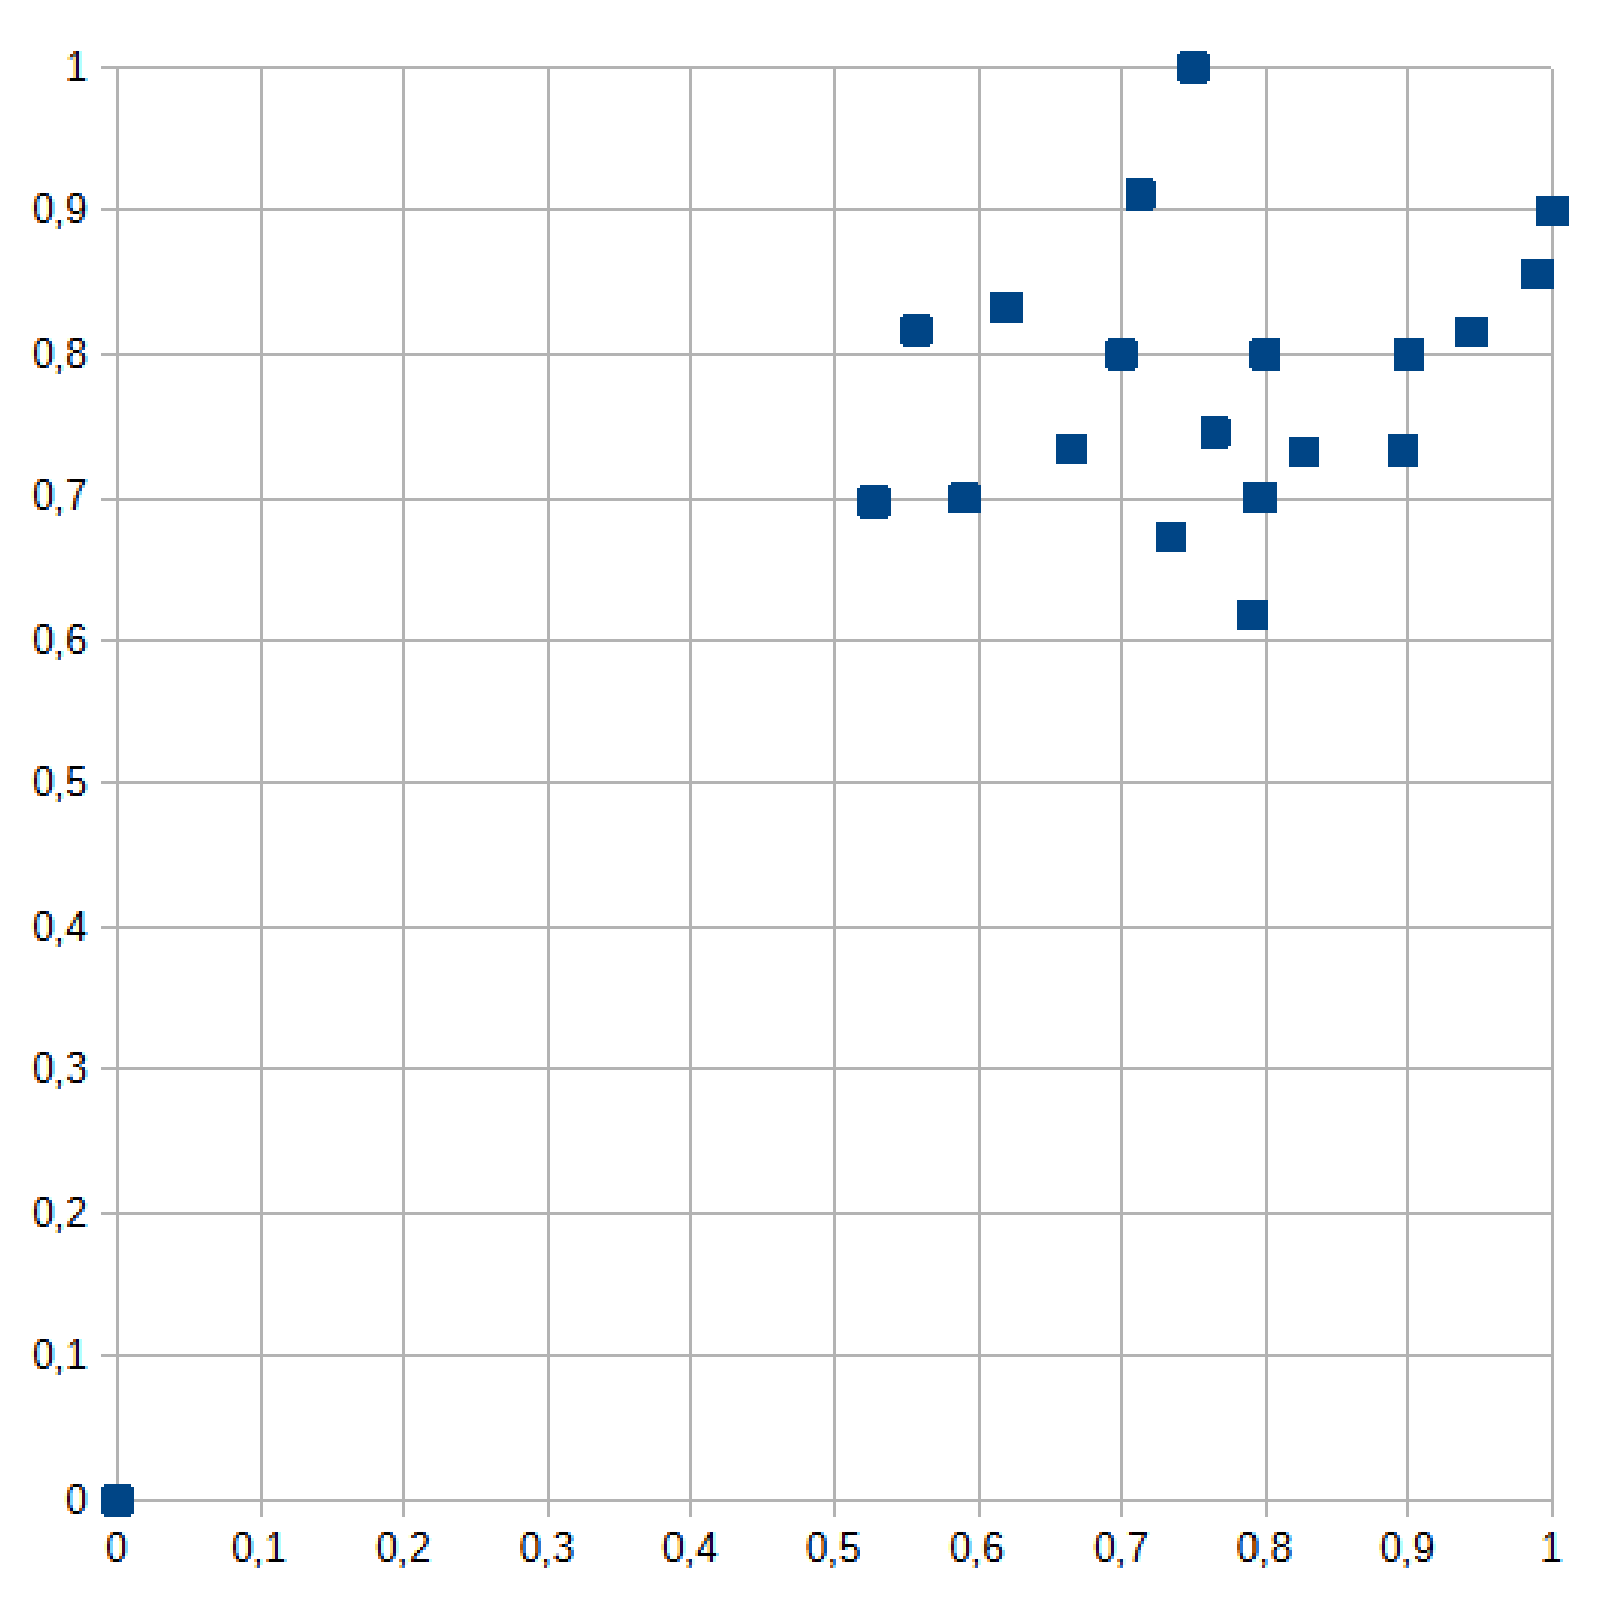
\includegraphics[width=\textwidth,height=4.6cm,keepaspectratio]{images/slide63_iforest_tree.png}
      \end{center}
    \end{column}
  \end{columns}
\end{frame}
